%% ===================================================================================
%% LaTeX Template for Academic Articles
%% Version: 2.0
%%
%% This template provides a clean, modern structure for academic articles
%% with proper formatting, citations, and professional appearance.
%% ===================================================================================

\documentclass[12pt, a4paper]{article}

%% ===================================================================================
%% PACKAGE IMPORTS
%% ===================================================================================

% -----------------------------------------------------------------------------------
% -- Font, Encoding, and Language
% -----------------------------------------------------------------------------------
\usepackage[T1]{fontenc}          % Use 8-bit T1 fonts
\usepackage[utf8]{inputenc}       % Allow utf-8 input
\usepackage[english,brazil]{babel} % Last language is the main one

% -----------------------------------------------------------------------------------
% -- Layout and Spacing
% -----------------------------------------------------------------------------------
\usepackage[
    left=3cm,
    right=2cm,
    top=3cm,
    bottom=2cm
]{geometry}                       % Set page margins
\usepackage{setspace}             % For line spacing control
\usepackage{fancyhdr}             % For headers and footers
\usepackage{titling}              % For better title control

% -----------------------------------------------------------------------------------
% -- Page Numbering Configuration
% -----------------------------------------------------------------------------------
\pagestyle{fancy}
\fancyhf{}                        % Clear all header and footer fields
\fancyhead[R]{\thepage}           % Page number on the top right
\renewcommand{\headrulewidth}{0pt} % Remove header line
\setlength{\headheight}{14.5pt}   % Fix fancyhdr warning

% Redefine plain page style to match fancy (fixes first page numbering)
\fancypagestyle{plain}{%
    \fancyhf{}
    \fancyhead[R]{\thepage}
    \renewcommand{\headrulewidth}{0pt}
}

% Reduce space before title
\setlength{\droptitle}{-60pt}

% -----------------------------------------------------------------------------------
% -- Author Block and Affiliations
% -----------------------------------------------------------------------------------
\usepackage{authblk}              % To handle multiple authors and affiliations

% -----------------------------------------------------------------------------------
% -- Graphics, Tables, and Code Listings
% -----------------------------------------------------------------------------------
\usepackage{graphicx}             % For including images
\usepackage{booktabs}             % For professional-quality tables
\usepackage{xcolor}               % For defining and using colors
\usepackage{listings}             % For code listings

% -----------------------------------------------------------------------------------
% -- Mathematics and Bibliography
% -----------------------------------------------------------------------------------
\usepackage{amsmath}              % For advanced math typesetting
\usepackage[round,authoryear]{natbib} % Citation management

% -----------------------------------------------------------------------------------
% -- Hyperlinks, Appendices, and Section Titles
% -----------------------------------------------------------------------------------
\usepackage{hyperref}             % For clickable links and PDF metadata
\usepackage[page]{appendix}       % For proper appendix handling (removed 'toc' option)
\usepackage{titlesec}             % For customizing section titles
%% ===================================================================================
%% CUSTOM COMMANDS AND CONFIGURATIONS
%% ===================================================================================

% -----------------------------------------------------------------------------------
% -- PDF Hyperlinks and Metadata
% -----------------------------------------------------------------------------------
\hypersetup{
    pdftitle={Comparação de Algoritmos de Busca Informada: A* vs. Busca Gulosa},
    pdfauthor={Caio A. S. Reis; Kariny M. P. Abrahão},
    colorlinks=true,
    linkcolor=blue!50!black,
    citecolor=green!50!black,
    urlcolor=blue!80!black,
    bookmarksopen=true,
    bookmarksnumbered=true
}
% -----------------------------------------------------------------------------------
% -- Section Title Formatting
% -----------------------------------------------------------------------------------
% Customize ALL section titles to be consistent and prevent awkward spacing.
\titleformat{\section}[block]
    {\normalfont\large\bfseries\raggedright} % Added \raggedright
    {\thesection}                            % The section number (e.g., "A")
    {1em}                                   % Space between number and title
    {}

% Also format starred sections (like \section*{Apêndices}) to match.
\titleformat{name=\section,numberless}[block]
    {\normalfont\large\bfseries\raggedright} % Added \raggedright
    {}
    {0em}
    {}
% -- Code Listing Style
% -----------------------------------------------------------------------------------
\lstset{
    numbers=left,
    numberstyle=\small\color{gray},
    frame=leftline,
    breaklines=true,
    basicstyle=\ttfamily\small,
    keywordstyle=\color{blue},
    commentstyle=\color{green!40!black},
    stringstyle=\color{purple},
    showstringspaces=false,
    tabsize=2,
    captionpos=b
}

%% ===================================================================================
%% ARTICLE METADATA
%% ===================================================================================
% [TODO: Fill in your article's information here]

\title{Comparação de Algoritmos de Busca Informada: A* vs. Busca Gulosa Aplicados a um Problema de Roteamento no Campus CTAN}
\author[1]{Caio A. S. Reis}
\author[2]{Kariny M. P. Abrahão}
\affil[1]{Departamento de Ciência da Computação, Universidade Federal de São João del-Rei (UFSJ)}
\date{\today}
% \affil[2]{Department of Electrical Engineering, Federal University of Somewhere}
\date{\today} % Or specify a date, e.g., \date{July 24, 2025}

%% ===================================================================================
%% DOCUMENT START
%% ===================================================================================
\begin{document}

\maketitle % Generates the title and author block

% -----------------------------------------------------------------------------------
% -- ABSTRACTS AND KEYWORDS
% -----------------------------------------------------------------------------------
\begin{abstract}
    \noindent Este trabalho modelou um problema de busca de caminho ótimo no Campus Tancredo Neves (CTAN) da UFSJ, representando-o como um grafo ponderado onde nós são locais de interesse e arestas correspondem às distâncias reais. Os algoritmos de busca informada A* e Busca Gulosa foram implementados em Python. Ambos foram aplicados para encontrar a rota entre dois pontos do campus. A análise demonstra que, embora a Busca Gulosa possa ser mais rápida em certos cenários, o A* garante a otimalidade do caminho encontrado, destacando o papel fundamental da função de custo real ($g(n)$) e de uma heurística admissível para a eficiência da busca.

    \vspace{\baselineskip}
    \noindent\textbf{Palavras-chave:} Inteligência Artificial; Busca A*; Busca Gulosa; Heurística; Otimização de Rota; NetworkX.
\end{abstract}

% -----------------------------------------------------------------------------------
% -- TABLE OF CONTENTS (Optional)
% -----------------------------------------------------------------------------------
% \tableofcontents % Uncomment this if you need a table of contents (for longer articles)
% \onehalfspacing % Example of changing line spacing after the abstracts/TOC

% -----------------------------------------------------------------------------------
% -- MAIN BODY OF THE ARTICLE
% -----------------------------------------------------------------------------------
\section{Introdução}

Este trabalho foca na implementação e comparação de dois algoritmos de busca informada aplicados a um problema prático de roteamento. O objetivo é:
\begin{enumerate}
    \item Modelar um problema de busca de caminho similar ao clássico problema da Romênia.
    \item Implementar os algoritmos de Busca Gulosa e A*.
    \item Aplicar os algoritmos ao modelo e comparar seus resultados, discutindo qual é mais eficiente e por quê.
\end{enumerate}

Para isso, escolhemos como cenário o Campus Universitário Tancredo Neves (CTAN), transformando um mapa geográfico em um grafo computacional para encontrar a rota de menor custo entre dois pontos.

\section{Modelagem do Problema}
O problema foi modelado como um grafo representando o Campus Universitário Tancredo Neves (CTAN). Cada nó do grafo corresponde a um local relevante (departamentos, biblioteca, etc.), enquanto cada aresta representa uma conexão viária. Os pesos atribuídos às arestas correspondem às distâncias em metros entre os locais, obtidas a partir do Google Maps. Essa abordagem garante que a busca por caminhos mais curtos corresponda a percursos realistas.

\begin{figure}[h!]
    \centering
    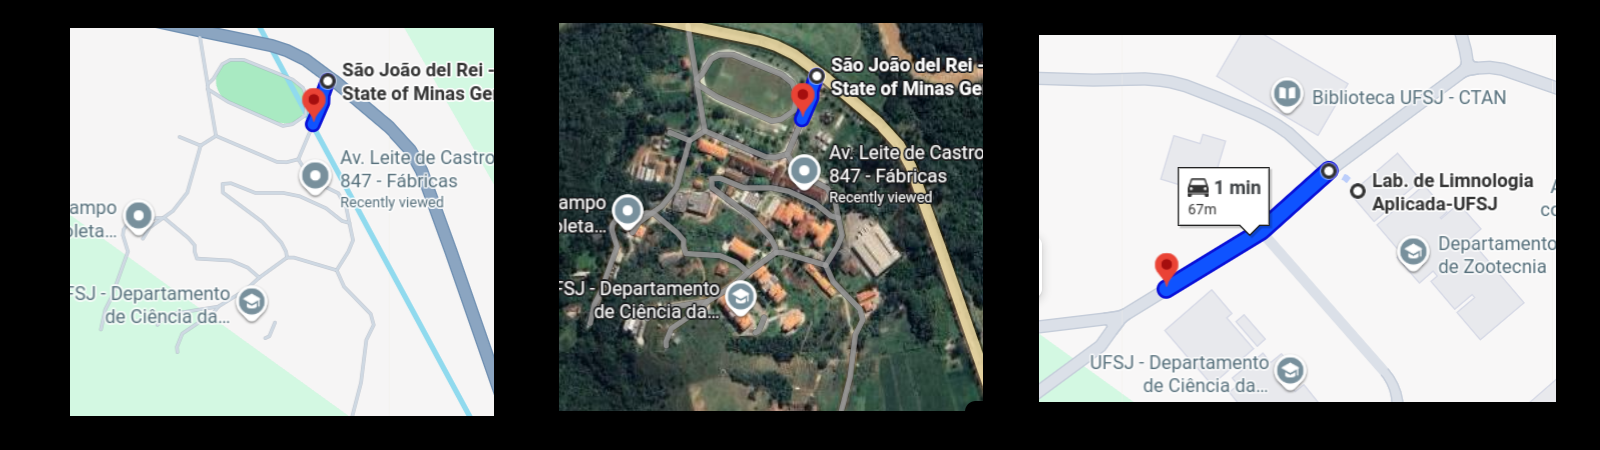
\includegraphics[width=0.8\textwidth]{../imgs/maps.png}
    \caption{Mapa do Campus CTAN utilizado como referência para a modelagem do grafo.}
    \label{fig:mapa_ctan}
\end{figure}

\section{Metodologia}

\subsection{Ferramentas e Tecnologias}
Para o desenvolvimento, utilizamos a linguagem **Python**. As seguintes bibliotecas foram essenciais:
\begin{itemize}
    \item \textbf{NetworkX}: Utilizada para a construção e manipulação do grafo do campus.
    \item \textbf{Heapq}: Biblioteca padrão do Python que implementa uma fila de prioridade, crucial para a eficiência da fronteira nos algoritmos de busca.
\end{itemize}

\subsection{Algoritmos Implementados}
Ambos os algoritmos utilizam uma função heurística, $h(n)$, que estima a distância de um nó $n$ até o objetivo.

\subsubsection{Busca Gulosa pela Melhor Escolha}
Este algoritmo expande o nó que parece estar mais próximo do objetivo, usando apenas a função heurística ($f(n) = h(n)$) para determinar a prioridade. Embora rápido, não garante encontrar a solução ótima.

\subsubsection{Busca A* (A-estrela)}
O A* equilibra o custo real do caminho percorrido desde o início até o nó atual, $g(n)$, com a estimativa heurística, $h(n)$. Sua função de avaliação é $f(n) = g(n) + h(n)$. O A* garante encontrar o caminho de menor custo, desde que a heurística seja **admissível** (nunca superestime o custo real).

\section{Estrutura e Execução do Projeto}
O código-fonte do projeto foi modularizado para separar as responsabilidades, facilitando a manutenção e o entendimento. A estrutura de arquivos é a seguinte:

\begin{verbatim}
/trabalho_ia/
|-- documentacao.pdf (Este documento)
|-- main.py (Script principal de execução)
|-- /src/
    |-- __init__.py (Torna src um pacote Python)
    |-- graph.py (Classe CampusGraph)
    |-- heuristic.py (Classe Heuristic)
    |-- search.py (Classes dos algoritmos de busca)
|-- /imgs/
    |-- maps.png (Imagem do mapa)
\end{verbatim}


Para executar o projeto, é necessário ter o pacote \texttt{networkx} instalado. Existem duas formas de garantir isso:

\begin{enumerate}
    \item \textbf{Instalação global} (disponível em qualquer terminal do sistema):
    \begin{verbatim}
    pip install networkx
    \end{verbatim}

    \item \textbf{Uso de ambiente virtual} (recomendado para isolar dependências):
    \begin{verbatim}
    python -m venv venv
    source venv/bin/activate      # Linux/macOS
    venv\Scripts\activate         # Windows
    pip install networkx
    \end{verbatim}
\end{enumerate}

Com o ambiente configurado, basta navegar até o diretório raiz do projeto (trabalho\_ia/) e executar o script principal:

\begin{verbatim}
python main.py
\end{verbatim}

O script irá:
\begin{itemize}
    \item Instanciar o grafo do campus universitário,
    \item Definir a heurística para os algoritmos,
    \item Aplicar a \textbf{Busca Gulosa pela Melhor Escolha} e o \textbf{A*},
    \item Imprimir os caminhos encontrados no console.
\end{itemize}

Dessa forma, é possível validar a implementação e comparar o comportamento dos dois algoritmos diretamente.

\section{Resultados e Análise Comparativa}


Definimos a "Entrada Estrada de Terra" como ponto de partida e o objetivo como "Entrada Principal BR". Nos primeiros testes realizados, ambos os algoritmos — \textbf{Busca Gulosa} e \textbf{A*} — retornaram o mesmo caminho, devido à heurística bem aproximada. Entretanto, com o objetivo de comparar o comportamento dos algoritmos, realizamos uma pequena modificação no grafo, de modo que eles encontrassem caminhos diferentes. Os resultados obtidos foram os seguintes:

\begin{itemize}
    \item \textbf{Busca Gulosa:} Encontrou um caminho com custo de 1200 metros.
    
    \textit{Caminho:} Entrada Estrada de Terra $\rightarrow$ Centro Pesquisa Queijos $\rightarrow$ ... $\rightarrow$ \textbf{Biblioteca} $\rightarrow$ ... $\rightarrow$ Entrada Principal BR

    \item \textbf{Busca A*:} Encontrou um caminho com custo de 1198 metros.
    
    \textit{Caminho:} Entrada Estrada de Terra $\rightarrow$ Centro Pesquisa Queijos $\rightarrow$ ... $\rightarrow$ \textbf{Departamento de Zootecnia} $\rightarrow$ ... $\rightarrow$ Entrada Principal BR
\end{itemize}

\subsection{Análise da Eficiência}
A Busca Gulosa, ao chegar no "Departamento de Geografia", escolheu ir para a "Biblioteca" (h=320) em vez do "Departamento de Zootecnia" (h=330), pois a primeira parecia mais promissora. No entanto, essa escolha levou a um caminho final 2 metros mais longo.

O A*, por outro lado, ao considerar o custo já percorrido ($g(n)$) em sua decisão, foi capaz de identificar que o caminho via "Departamento de Zootecnia" era, de fato, o mais curto.

O algoritmo \textbf{A*} demonstrou \textbf{garantir a otimalidade}. A Busca Gulosa pode ser mais rápida em termos de número de comparações, mas arrisca encontrar soluções subótimas. A superioridade do A* reside em sua capacidade de balancear o custo real com a estimativa futura para tomar decisões mais bem informadas.

\section{Conclusão}
Este trabalho demonstrou a aplicação de algoritmos de busca informada em um problema de roteamento do mundo real. A comparação entre a Busca Gulosa e o A* confirmou a teoria: enquanto a Busca Gulosa oferece uma solução rápida, mas não necessariamente ótima, o A* garante encontrar o caminho de menor custo ao incorporar o custo já percorrido em sua função de avaliação. Para aplicações onde a otimalidade é crucial, o A* é comprovadamente o método mais eficiente e robusto.
% -----------------------------------------------------------------------------------
% -- POST-TEXTUAL ELEMENTS
% -----------------------------------------------------------------------------------

% --- Bibliography ---
% \bibliographystyle{plainnat}
% \bibliography{references}

% The \appendix command switches from numbered sections (1, 2, 3) to lettered
% sections (A, B, C) for all subsequent \section commands. It only needs to be
% called once.
% \appendix
% \cleardoublepage

% -----------------------------------------------------------------
% -- Block 1: APÊNDICES (Optional)
% -- If you have no appendices, DELETE this entire block.
% -----------------------------------------------------------------
% \phantomsection
% \section*{Apêndices}
% \addcontentsline{toc}{section}{Apêndices} % Adds a non-clickable title to the TOC

% \section{Supplementary Data}
% \label{app:data}
% This is the first appendix. It will be labeled "Apêndice A".

% \section{Source Code Listing}
% \label{app:code}
% This is the second appendix, labeled "Apêndice B".

% -----------------------------------------------------------------
% -- Block 2: ANEXOS (ATTACHMENTS) (Optional)
% -- If you have no attachments, DELETE this entire block.
% -----------------------------------------------------------------
% \cleardoublepage % Optional: start attachments on a new page for a clean break.
% \phantomsection

% Change the name from "Apêndice" to "Anexo" for the sections that follow.
% \renewcommand{\appendixname}{Anexo}

% \section*{Anexos}
% \addcontentsline{toc}{section}{Anexos} % Adds a non-clickable title to the TOC

% \section{Datasheet for Sensor XYZ}
% \label{anx:datasheet}
% This is the first attachment. Its label will correctly be "Anexo C" if you
% also have appendices, or "Anexo A" if you deleted the appendix block.

% \section{Technical Specifications}
% \label{anx:specs}
% This is the second attachment, labeled "Anexo D".

\end{document}